\documentclass[margin,line,a4paper]{resume}
 
\usepackage[latin1]{inputenc}
\usepackage[english,danish]{babel}
\usepackage[utf8]{fontenc}
\usepackage[none]{hyphenat}
\usepackage{graphicx,wrapfig}
\usepackage{url}
\usepackage[colorlinks=true, a4paper=true, pdfstartview=FitV,
linkcolor=blue, citecolor=blue, urlcolor=blue]{hyperref}
\pdfcompresslevel=9
\frenchspacing
 
\begin{document}
\raggetright
{\sc \Large Curriculum Vitae -- Martin Bjeldbak Madsen}
\begin{resume}
    \vspace{0.5cm}
    \begin{wrapfigure}{R}{0.6\textwidth}
         \vspace{-1cm}
        \begin{center}
        \reflectbox{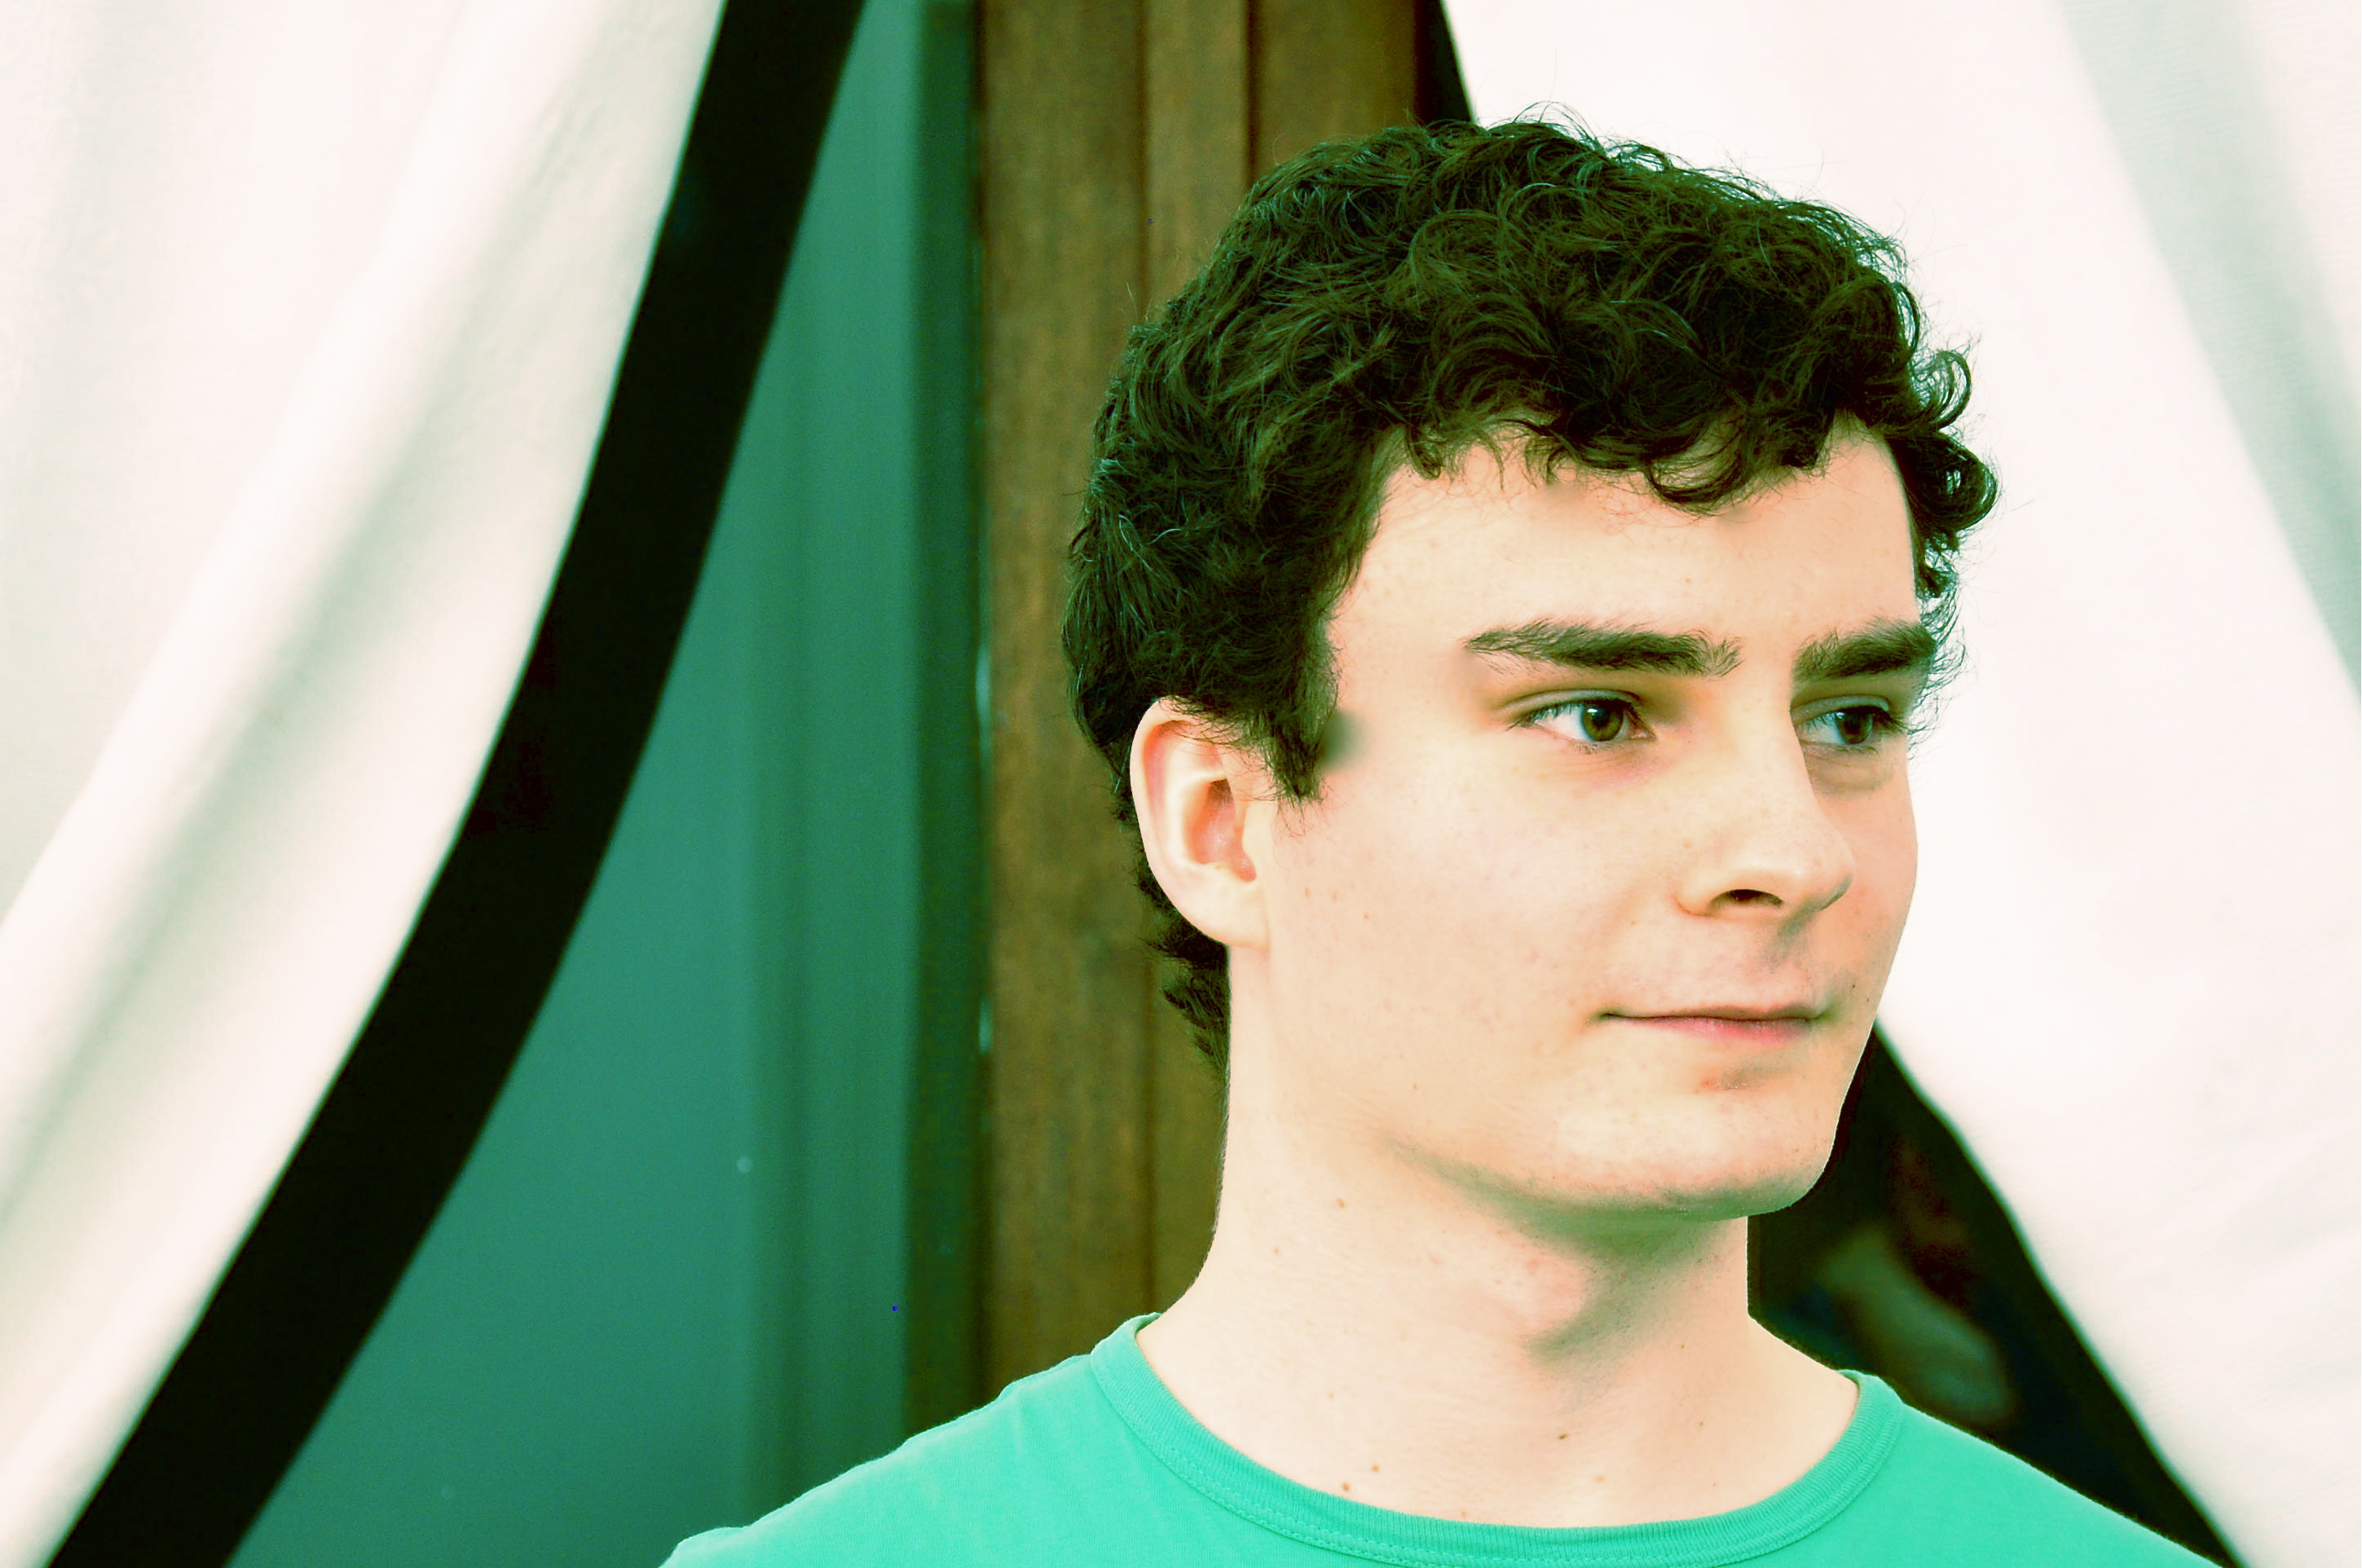
\includegraphics[width=0.6\textwidth]{DSC_0056_2.JPG}}
        \end{center}
         \vspace{-2cm}
    \end{wrapfigure}

    \section{\mysidestyle Personlige\\Information}%\vspace{2mm}
    Martin B. Madsen\\
    9. juni 1992 (20 �r)\\ \\
    Toldstrupsgade 20, 3, -1\\
    9000 Aalborg\\
    Danmark\\
    Mobil: 26 27 36 60\\
    \href{mailto:martin2madsen@gmail.com}{martin2madsen@gmail.com}\\
    \href{http://www.martinbmadsen.dk}{martinbmadsen.dk}\\
    \href{http://dk.linkedin.com/pub/martin-madsen/21/9b0/b0}{LinkedIn - Martin Madsen}\vspace{1cm}

    F�dt og opvokset i Danmark til jeg var 5 �r, hvorefter vi havde et
    9-�r langt ophold i udlandet, i b�de England og USA, s� jeg er vant til
    at tale engelsk og dansk med de lokale, samt tilpasse mig til nye milj�er. Jeg
    bor selvst�ndigt og vil gerne arbjede inden for computere eller med mennesker i it-branchen som et supplement til mit studie.

    I �jeblikket studerer jeg Datalogi p� Aalborg Universitet. Her g�r
    jeg p� 2. semester og engagerer mig i nogle sp�ndende
    projekter baseret p� en dynamisk grundlag bygget op p� problembaseret gruppearbejde!

    Jeg har dansk k�rekort til bil.

    \section{\mysidestyle Uddannelse} \textbf{Aalborg Universitet - Kandidat i Datalogi}
    (2011 - 2016) Jeg afslutter 2. semester i juni 2012.

    \textbf{EUC Nord - HTX} (2008 - 2011) Teknisk gymnasium i Hj�rring. Naturvidenskabelig
    linje (Matematik A, Fysik A).

    \textbf{Bagterpskolen} (2006 - 2008) Folkeskole i Hj�rring.

    \textbf{J. R. Gerrits Middle School}
    (2003 - 2006) Elementary og Middle School i Kimberly,
    Wisconsin, USA.

\section{\mysidestyle Professionel erfaring}\vspace{1mm}
\begin{description}

  \item[2010 sept $\rightarrow$ nu] Startede enkeltmandsvirksomheden
    \emph{Divambu}. Virksomheden har fokus p� udvikling og hosting af
    hjemmesider samt konsultentservicer inden for IT og computere. P�
    \url{divambu.dk} ses en portfolio af projekter jeg har gennemf�rt
    for kunder.

  \item[2009 feb $\rightarrow$ 2010 jun] Ungarbejder ved Fakta
    a/s. Jobfunktionerne bestod i at side ved kassen, fylde varer op,
    ordne dagligdags butiksarbejde, osv. Meget af jobbet bestod af at have
    kontakt med kunderne, forst� deres problem, og derefter l�se det.

\end{description}
\pagebreak

\section{\mysidestyle Computer-kompetencer}\vspace{1mm} Jeg kan
hurtigt s�tte mig ind i noget nyt, men der er nogle s�rlige emner, der
interesserer mig mest og vil blive listede her:
\vspace{0.5cm}
\begin{description}

  \item[Operativ-systemer] Grundl�ggende forst�else for de fleste
    typer af Linux: Ubuntu, Debian, CentOS og Arch Linux; Microsoft
    Windows og til en hvis grad: Mac OS X.
  \item[Servere og databaser] Nginx/Apache, openSSH, CUPS, MySQL.

  \item[CMS-systemer] Wordpress, phpBB, til en mindre grad: Drupal.

  \item[Programmering-, scription- og markupssprog] Bash, \LaTeX,
    HTML, CSS, C, C\#, Javascript og kendskab til \& jQuery, node.js og Python.

\end{description}

\section{\mysidestyle Sproglige kompetencer}
Mit modersm�l er dansk, men n�sten alt det jeg laver er p� engelsk,
b�de i forbindelse med computere men ogs� kommunikationen med
internationale venner, samt i en akademisk forstand p� universitetet.

\textbf{Dansk:} modersm�l\\
\textbf{Engelsk sprogligt:} flydende\\
\textbf{Engelsk skriftligt:} flydende\\
\textbf{Engelsk l�seforstand:} h�j\\

\section{\mysidestyle Interesser}

N�r jeg ikke sidder forand computeren, elsker jeg at nyde jeg en kop 
te med en god bog i h�nden. Der er heller ikke noget
mere sp�ndende i livet end at tage ud i verden for at rejse rundt uden
for trykke Danmark. Heldigvis har jeg fundet nogle gode venner i udlandet, som jeg engang imellem f�r forn�jelsen at bes�ge! Jeg er ogs� stor tilh�nger af elektronisk musik som trance og elektronika, dog kan jeg engang imellem godt finde p� at leje lidt rundt med nogle dubstep numre i Fruity Loops. Udover dette nyder jeg ogs� at lave friskt og gr�nt mad, der kan f� en til at savle!


\end{resume}
\end{document}
